\documentclass[11pt, oneside]{article}   	% use "amsart" instead of "article" for AMSLaTeX format
\usepackage{geometry}                		% See geometry.pdf to learn the layout options. There are lots.
\geometry{letterpaper}                   		% ... or a4paper or a5paper or ... 
%\geometry{landscape}                		% Activate for for rotated page geometry
%\usepackage[parfill]{parskip}    		% Activate to begin paragraphs with an empty line rather than an indent
\usepackage{graphicx}				% Use pdf, png, jpg, or eps� with pdflatex; use eps in DVI mode
								% TeX will automatically convert eps --> pdf in pdflatex		
\usepackage{amssymb}
\usepackage{amsmath}

\title{Analysis of Book Pull}
%\date{}							% Activate to display a given date or no date

\begin{document}
\maketitle
%\section{}
%\subsection{}

We would like to analyze the stability of a book that is being pivoted about one of its corners.  We parameterize the problem using two variables:
\begin{enumerate}
\item $d$ - Represents the distance of the pivot point from an arbitrary point - in most cases, the starting location of that pivot point.
\item $\theta$ - Represents the angle of the pivot.
\end{enumerate}

\begin{figure}[h]
\begin{center}
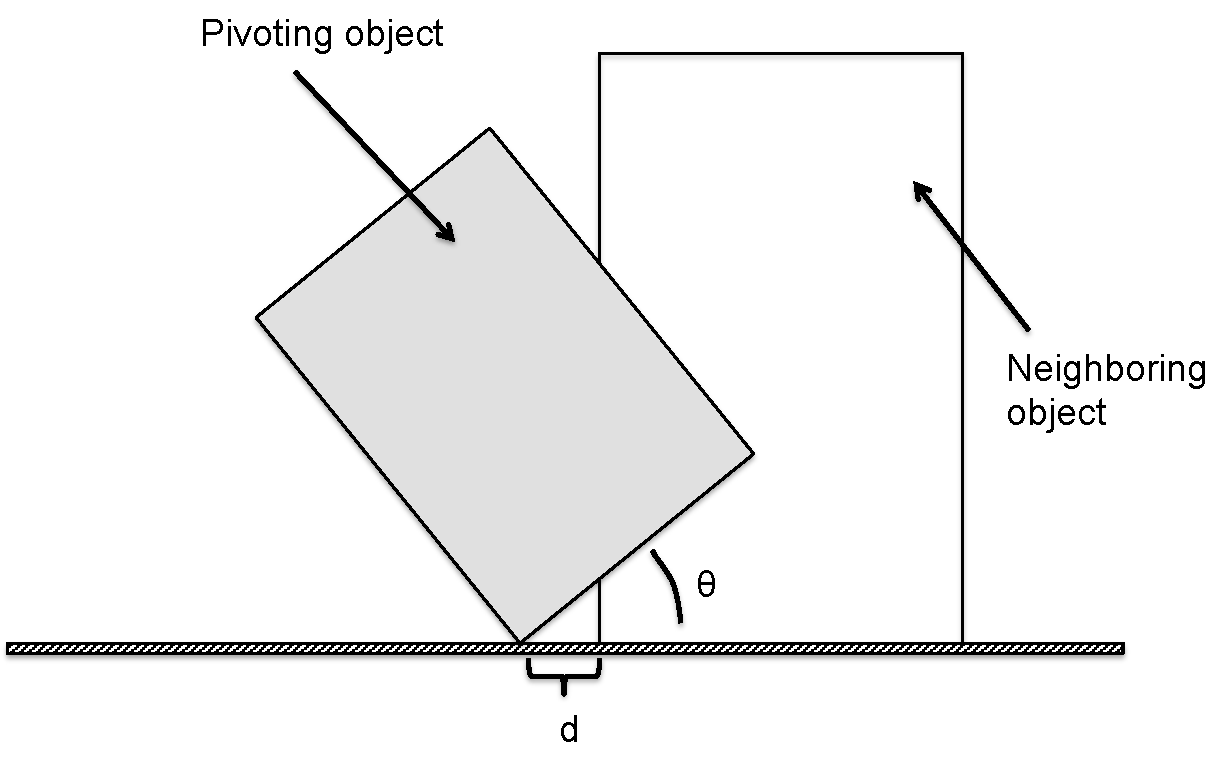
\includegraphics[width=0.5\textwidth]{figs/pull_parameters}
\end{center}
\label{figs:pull_parameters}
\end{figure}
Figure ~\ref{figs:pull_parameters} shows highlights these two parameters.

We are interested in determining if the moment imparted on the pivoting book by the neighboring objects is enough to balance the moment caused by gravity. We can calculate the moment from gravity as:
\[ mg \times p_{com} \]
where $m$ is the mass of the book and $p_{com}$ is the vector from the pivot point to the center of mass.

\begin{figure}[h]
\begin{center}
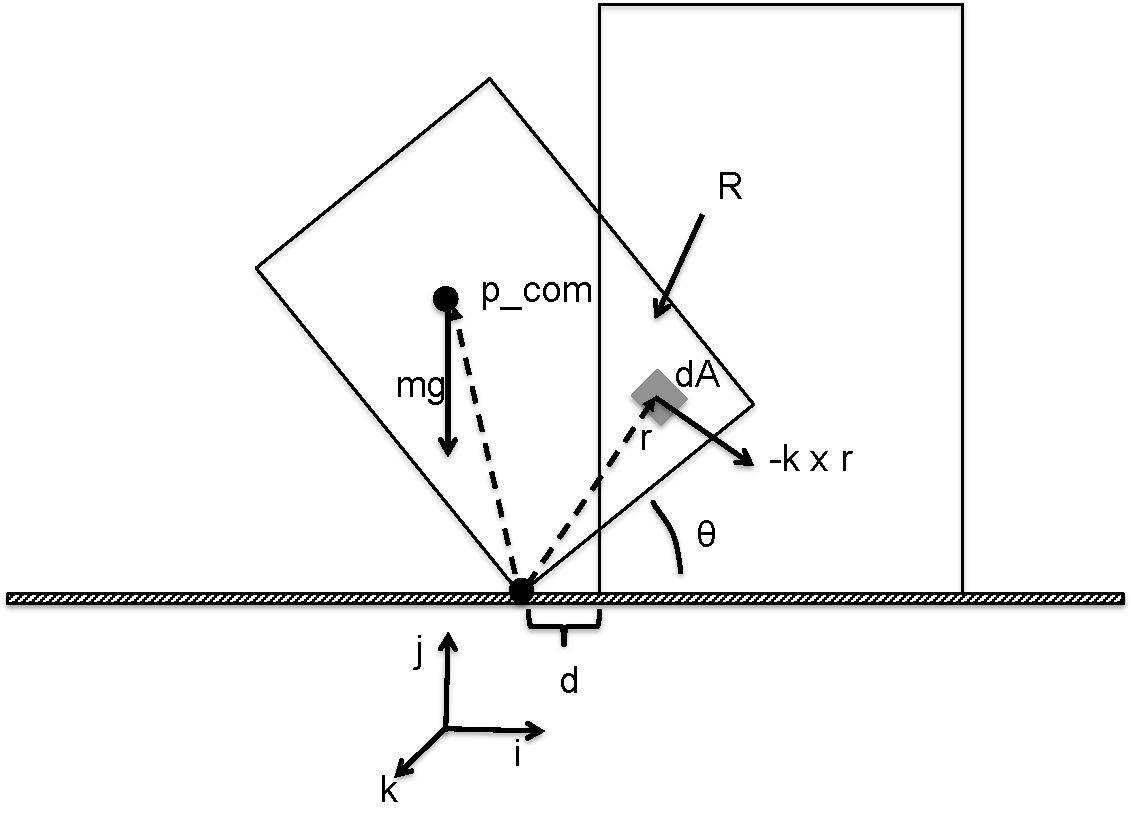
\includegraphics[width=0.8\textwidth]{figs/patch_moment}
\end{center}
\label{figs:patch_moment}
\end{figure}
To calculate the moment imparted by neighboring objects, we look at the cross section of the book that is in contact with those objects.  Call this $R$.  Then, for a particular patch, $dA$, within that cross section, we can compute the moment as follows:
\[ r \times (-\hat{k} \times r)\textbf{ }p\textbf{ }dA \]
To calculate the total moment we integrate over the entire region $R$:
\[ \int_R r \times (-\hat{k} \times r)\textbf{ }p\textbf{ }dA \]
where $r$ is the distance from the pivot point to the patch, $p$ is the pressure distribution, and $dA$ represents the patch.  Figure \ref{figs:patch_moment} shows these parameter.

Then we can check stability by checking whether the following inequality holds:
\begin{equation}
mg \times p_{com} \leq \int_R r \times (-\hat{k} \times r)\textbf{ }p\textbf{ }dA 
\label{eq:stability}
\end{equation}

We can break down the integral into the following:
\[ \int_r \|r\| \int_{\phi} I_{inside}(d, \theta) \textbf{ }p\textbf{ }dA\textbf{ }d\phi\textbf{ }dr \]
Here $I_{inside}$ is an indicator function such that is 1 when $dA$ is inside R and 0 otherwise.   Here our patches are arc segments with area defined by:
\[dA = d\phi\textbf{ }\pi r^2 - d\phi\textbf{ }\pi (r - dr)^2 \]
Where $d\phi$ represents the discretization size in the $\phi$ dimension, and $dr$ represents the discretization size in the $r$ dimension.

Since $dA$ is defined by parameters in the book frame, we can precompute these patches offline.  Then online computation of the moment involves only computing the mask, $I_{inside}$, and a table lookup. 

$I_{inside}$ is a function of the parameters of our scene $(d, \theta)$.  We can vary those parameters and  compute the inequality in equation~\ref{eq:stability}, then generate a map of the stability regions in terms of $d$ and $\theta$. 
\end{document}  